\documentclass[a4paper, 12pt]{article}
\usepackage[T2A]{fontenc}
\usepackage[utf8]{inputenc}
\usepackage[english,russian]{babel}
\usepackage{amsmath, amsfonts, amssymb, amsthm, mathtools, misccorr, indentfirst, multirow}
\usepackage{wrapfig}
\usepackage{graphicx}
\usepackage{subfig}
\usepackage{adjustbox}
\usepackage{pgfplots}
\usepackage{mathrsfs}

\usepackage{geometry}
\geometry{top=20mm}
\geometry{bottom=20mm}
\geometry{left=20mm}
\geometry{right=20mm}
\newcommand{\angstrom}{\textup{\AA}}

\begin{document}
    \title{Влияние параметров периодического потенциала на спектр состояний и на возникновение запрещенной зоны в модели Кронига-Пенни}
    \author{Нехаев Александр 654 гр.}
    \maketitle
    \section{Периодическая задача}
    Рассмотрим одномерную решетку ионов, расстояние между которыми $a$. Потенциал при этом будет периодическим, его вид приведен на рис. \ref{fig:one}.
    \begin{figure}[h]
        \centering
        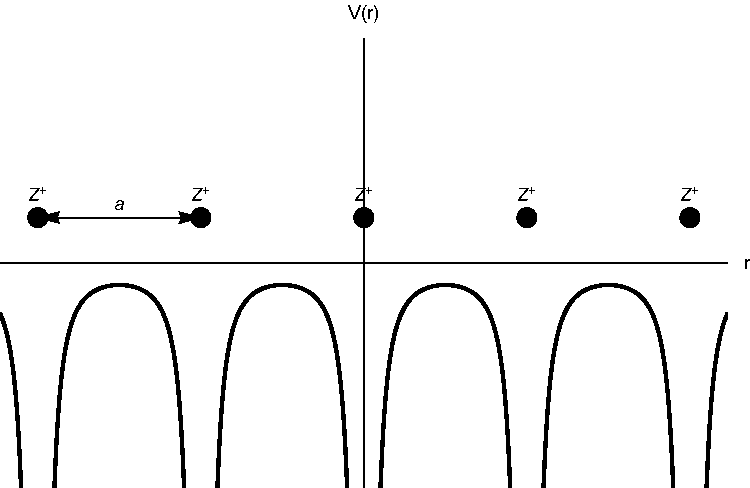
\includegraphics{fig1.pdf}
        \caption{Пример периодического потенциала}
        \label{fig:one}
    \end{figure}

    Рассмотрим идеализированный случай бесконечного кристалла. Уравнение Шрёдингера имеет вид:
    \begin{equation}
        -\frac{\hbar^2}{2m}\frac{\partial^2\psi(x)}{\partial x^2}+V_a(x)\psi(x)=E\psi(x)
    \end{equation}
    с периодическим потенциалом $V_a(x)=V_a(x+a)$. Спектр определяется как множество тех энергий, при которых уравнение имеет решения, ограниченные на всей вещественной оси.
    \section{Теорема Блоха}
    Собственные состояния одноэлектронного гамильтониана
    \begin{equation}
        \hat{H}=-\frac{\hbar^2}{2m}\nabla^2+V(\bf{r}),
    \end{equation}
    где потенциал $V(\bf{r})$ периодичен по всем векторам $\bf{R}$ решетки Бравэ, могут быть выбраны таким образом, чтобы их волновые функции имели форму плоской волны, умноженной на функцию, обладающую той же периодичностью, то и решетка Бравэ:
    \begin{equation}
        \psi_{n\bf{k}}=e^{i\bf{kr}}u_{n\bf{k}}(\bf{r}),
    \end{equation}
    где $u_{n\bf{k}}({\bf{r}+\bf{R}})=u_{n\bf{k}}(\bf{r})$, для всех $\bf{R}$, принадлежащих решетке Бравэ. Электронные волновые функции в виде $u_{n\bf{k}}({\bf{r}})=u_{n{\bf{k}}}(\bf{r+R})$ называют функциями Блоха.
    \section{Модель Кронига-Пенни}
    Для упрощения задачи потенциал приближают прямоугольным, используя теорему Блоха (рис. \ref{fig:two}).
    \begin{figure}[h]
        \centering
        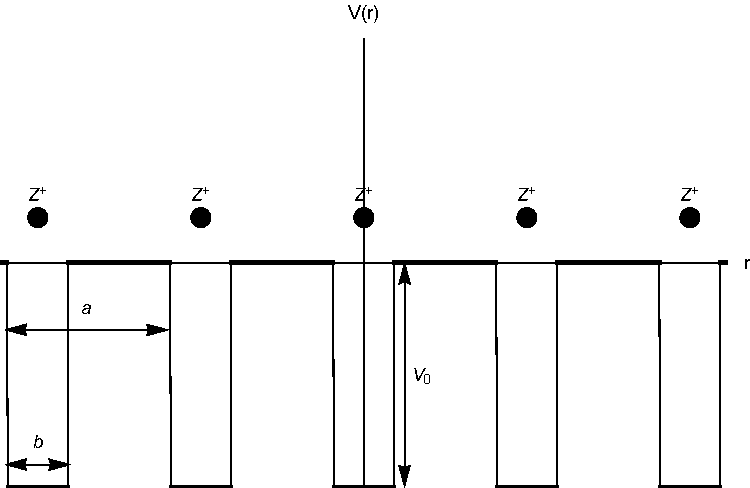
\includegraphics{fig2.pdf}
        \caption{Периодический потенциал с периодом $a$ и шириной прямоугольной ямы $b$}
        \label{fig:two}
    \end{figure}
\end{document}